\begin{frame}{%
  \begin{minipage}[t]{0.32\textwidth}
    Toppet skallesluger
  \end{minipage}%
  \hfill
  \begin{minipage}[t]{0.36\textwidth}
    \centering
    \footnotesize\textbf{Jagttid:} Ingen jagttid
  \end{minipage}%
  \hfill
  \begin{minipage}[t]{0.15\textwidth}
    \noindent\raggedleft
    
\includegraphics[width=0.5cm, height=0.5cm, keepaspectratio]{Billeder/Ikoner/star.png}%
    \hspace{0.2em}%
    
\includegraphics[width=0.5cm, height=0.5cm, keepaspectratio]{Billeder/Ikoner/star.png}
  \end{minipage}%
} % Ændret: Højre minipage nu med begge ikoner side om side
  \vspace{0.25em}
  \begin{columns}[T]
    % --- Venstre kolonne: Tekst ---
    \column{0.55\textwidth}
    \setlength{\parskip}{0.5em}
    \small
    \RaggedRight\textbf{\textit{Mergus serrator}} – lang slank dykand \par

    \textbf{Udseende:} \\
    \quad – Andrik: metalgrønt hoved, røde øjne, hvid halsring, langt næb \\
    \quad – And: spraglet grå med langt tyndt næb \par

    \textbf{Levesteder:} \\
    \quad – Kyster og fjorde

    \textbf{Føde:} \\
    \quad – Småfisk og krebsdyr \par

    \textbf{Udbredelse:} \\
    \quad – Hele Danmark \par

    \textbf{Træk/standfugl} \\
    \quad – Begge \par

    % --- Højre kolonne: To billeder stablet over hinanden (større størrelse) ---
    \column{0.40\textwidth}
    \centering
    \fbox{%
      \begin{minipage}{\linewidth}
        \centering
        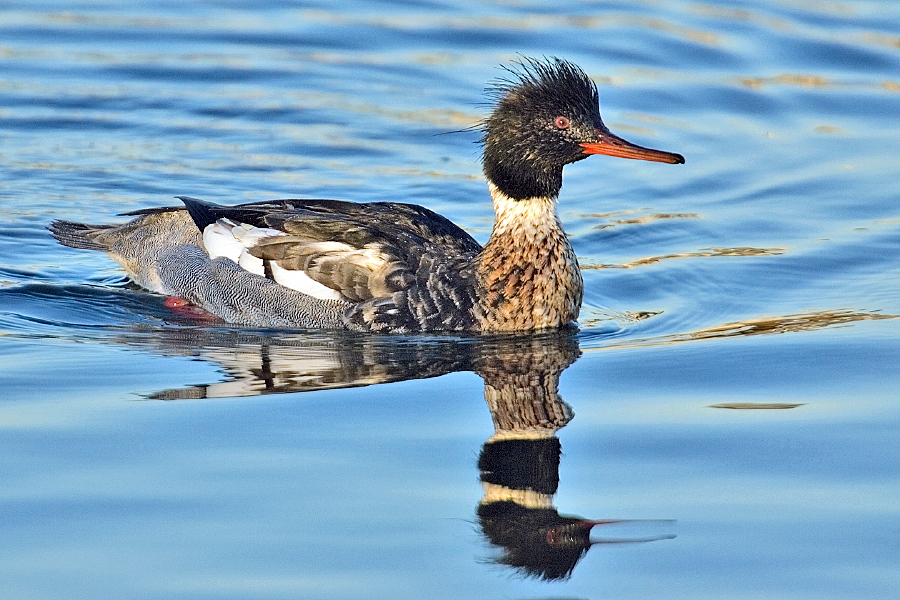
\includegraphics[width=0.8\linewidth, height=3.5cm, keepaspectratio]{Billeder/Dyr/Fugle/Skalleslugere/toppet_skallesluger_han.jpg}\\[0.5em]
        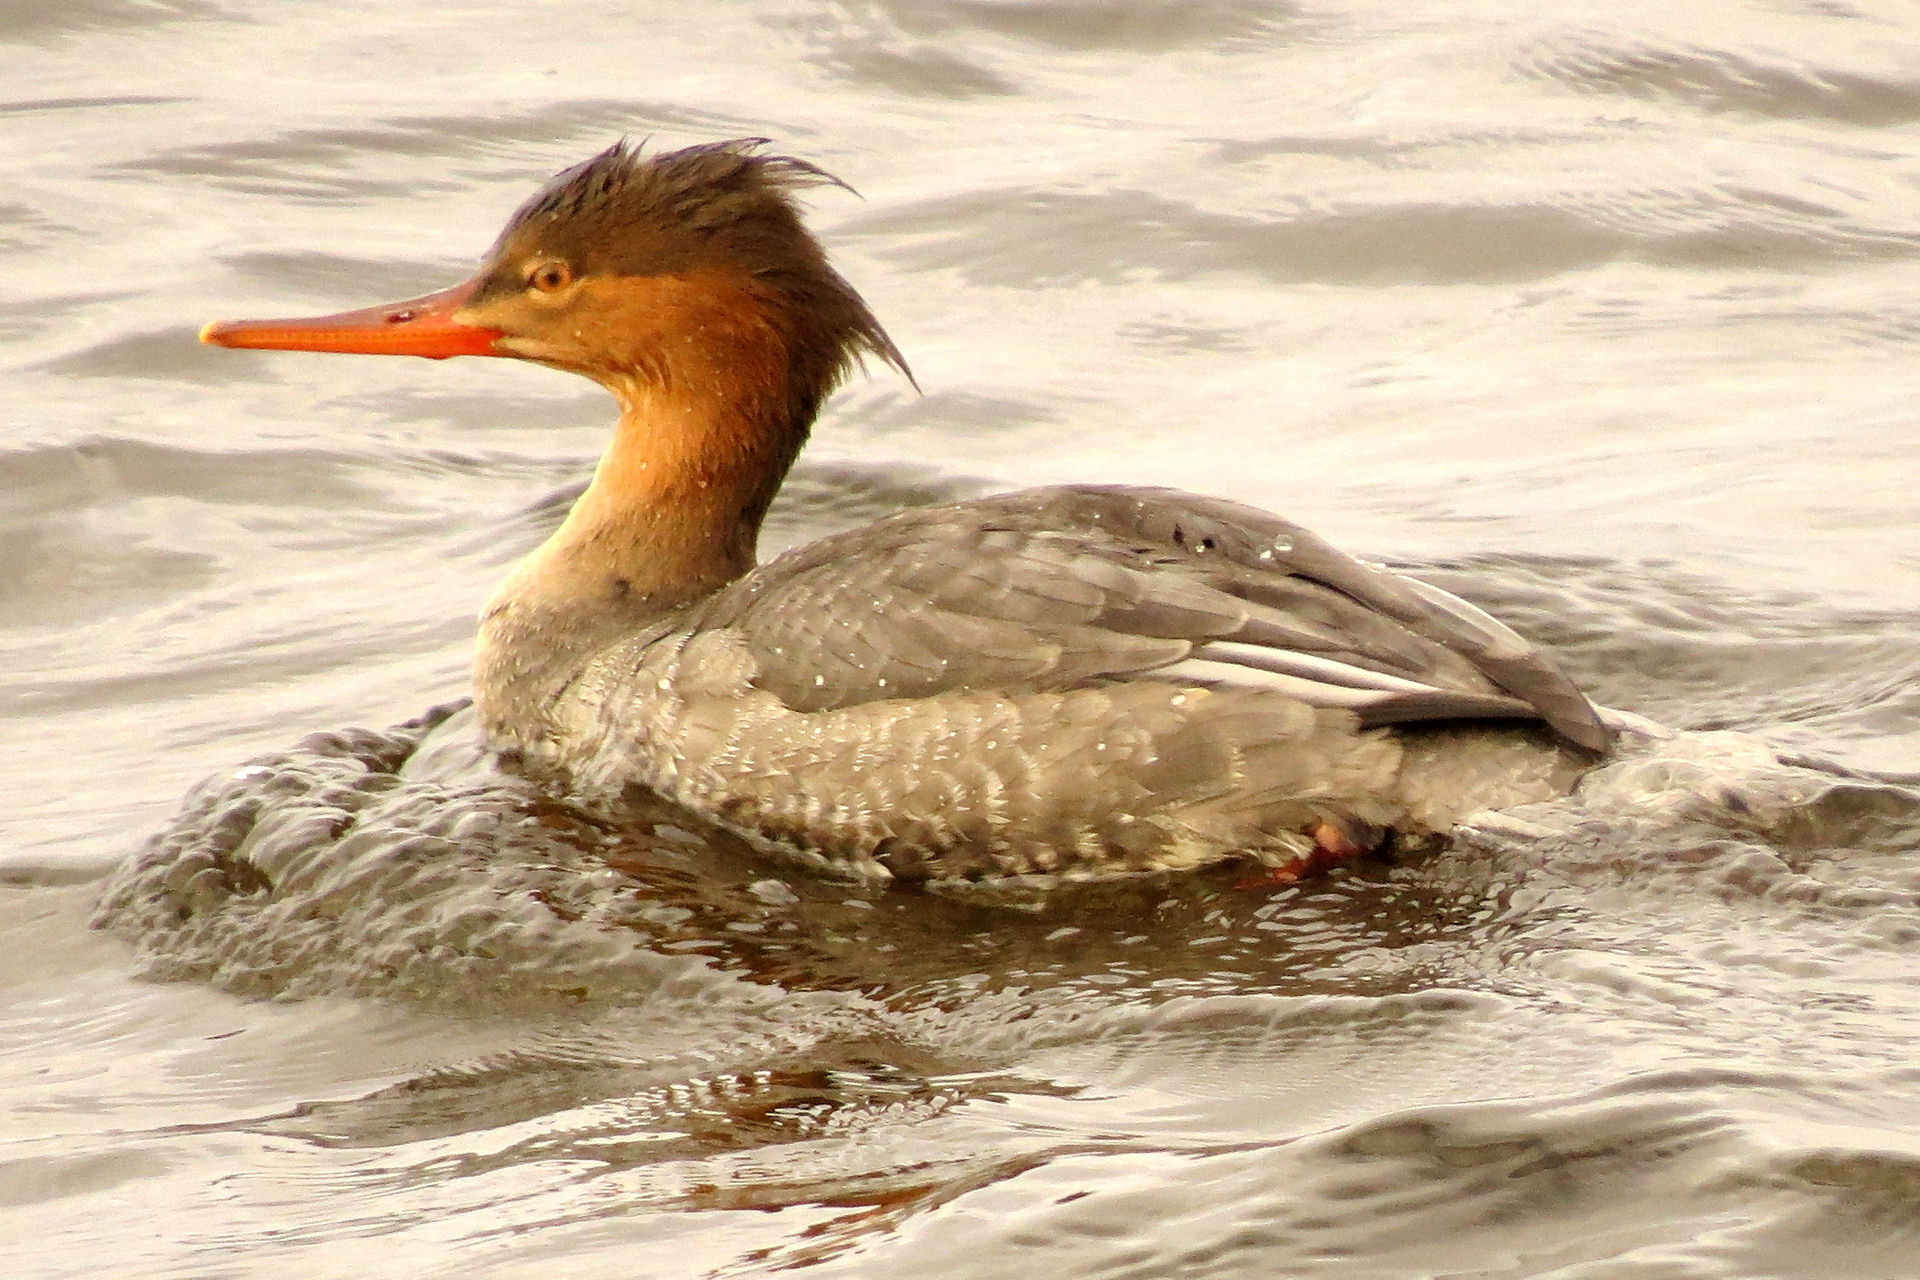
\includegraphics[width=0.8\linewidth, height=3.0cm, keepaspectratio]{Billeder/Dyr/Fugle/Skalleslugere/toppet_skallesluger_hun.jpg}%
      \end{minipage}
    }%
    \vspace{0.05em}
    \footnotesize Andrik øverst, and nederst
  \end{columns}
\end{frame}